\documentclass[a4paper]{article}

\usepackage[english]{babel}
\usepackage[utf8]{inputenc}
\usepackage{fullpage}
\usepackage{amsmath}
\usepackage{graphicx}
\usepackage[colorinlistoftodos]{todonotes}
\usepackage{hyperref}
\usepackage{amssymb}
\usepackage{outline} \usepackage{pmgraph} \usepackage[normalem]{ulem}
\usepackage{graphicx} \usepackage{verbatim}
\usepackage{amssymb} %checklist

\usepackage{wasysym} %checkedbox
\definecolor{mypink1}{rgb}{0.858, 0.188, 0.478}
\definecolor{mypink2}{RGB}{219, 48, 122}
\definecolor{mypink3}{cmyk}{0, 0.7808, 0.4429, 0.1412}
\definecolor{mygray}{gray}{0.4}
 

%\usepackage[dvipsnames]{xcolor} 

% \usepackage{minted} % need `-shell-escape' argument for local compile

\title{
    \vspace*{1in}
    
\includegraphics[width=3.25in]{figures/uff-logo.png} \\
    \vspace*{1.2in}
    % \textbf{\huge Weekly Report.}
    \textbf{\huge Report.}
    \vspace{0.2in}\\
    \vspace{0.2in}
}

\author{Luigy Machaca \\
    %\vspace*{0.5in} \\
    \textbf{luigyarcana@id.uff.br} \\
    % \vspace*{1in}
}

\date{\today}


\begin{document}

\maketitle
\setcounter{page}{0}
\thispagestyle{empty}
\newpage


\section{Research Project}
In this project, we will develop a framework system that is a blend that combines object detection, visual object tracking, and one-class classification. This job aims to generate a set of track fragments of each person in the video. Each item is called a tracklet, and a collection of tracklets we called a gallery. Additionally, each of the gallery's tracklets involves the best representative candidate.

The framework commits a squeezing of the number of queries that will provide to the re-identification algorithm. We will explain these details more later.

The input of the framework is simple raw video. For this test we use a \textbf{TownCentre} video with the following properties.
\begin{enumerate}
    \item Frames per second = 25 FPS.
    \item Number of frames = 7500 frames.
    
    \item Duration of video = 5 minutes 0 seconds
    \item Resolution of video = 1920 * 1080
\end{enumerate}

\subsection{Framework Architecture}

We split this framework into two blocks, where the first part supports the generate tracklets and the second part chooses the best candidate or candidates. 








% #####

The framework consist in consists of a hybrid of online and offline tracking algorithm is applicable to areas such as object tracking surveillance videos or semi-autonomous cameras technology \cite{re3}.



It is applicable to areas as a stand-alone camera system or one that could easily be embedded into an even larger system. This report expressed how has been to development since august.


\subsection{Algorithm}
%\subsection{\textcolor{mygray}{Algorithm}}
\subsubsection{Re3: Real-Time Recurrent Regression Networks for Visual Tracking of Generic Objects.}
%\subsubsection{\textcolor{mygray}{Re3: Real-Time Recurrent Regression Networks for Visual Tracking of Generic Objects.}

%\iffalse
The tracking pipeline, consists of:
\begin{itemize}
    \item convolutional layers to embed the object appearance, 
    \item recurrent layers to remember appearance and motion information, 
    \item and a regression layer to output the location for the object. 
\end{itemize}
See Figure \ref{fig:re3}

\begin{figure}[hb]
    \centering
    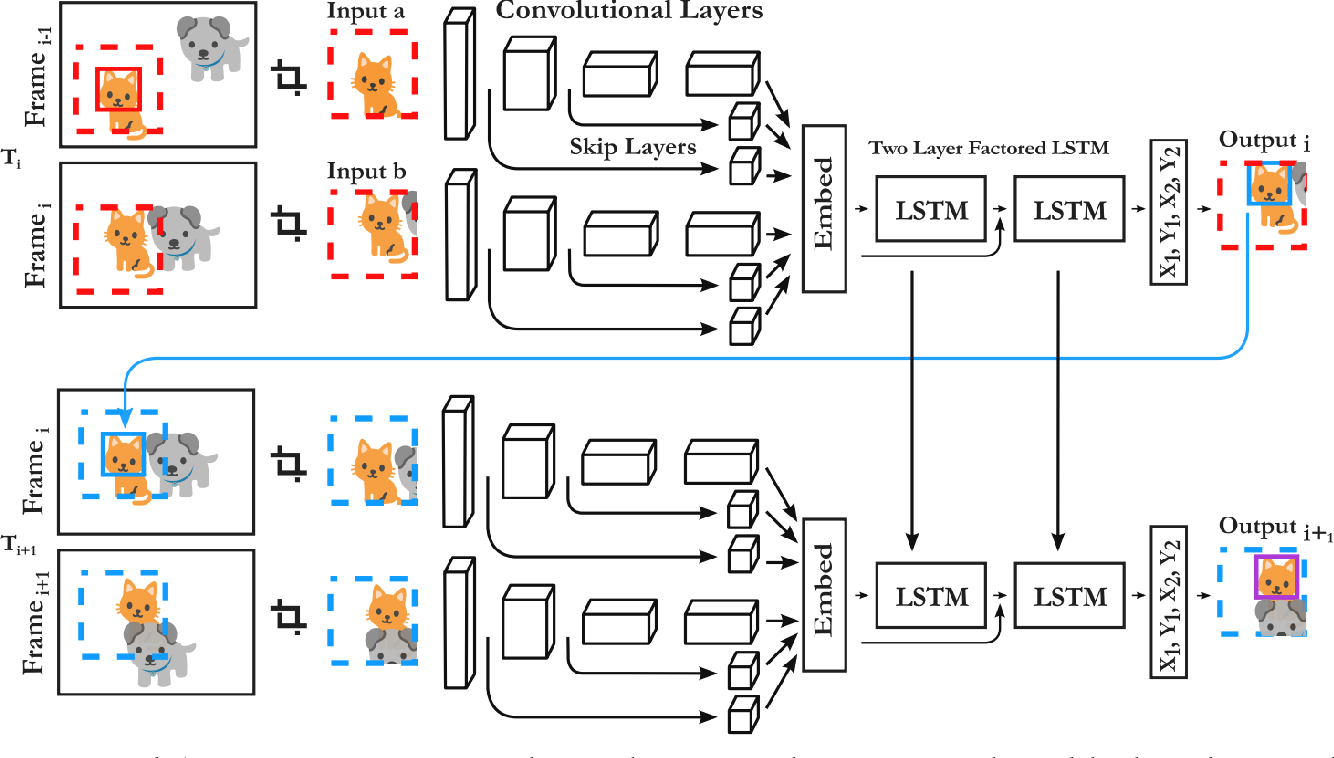
\includegraphics[width=0.6\textwidth]{figures/pipeline-re3.png}
    \caption{
            cccccccccc
    }
    \label{fig:re3}
    \medskip
    \small 
        \begin{itemize}
        \item Image crop pairs are fed in at each time step.
        \item Both crops are centered around the object\'s location in the previous frame 
        \item and padded to two times the width and height of the object. 
        \item before every pooling state, to add a skip layer to preserve high-resolution spatial information.
        \item The weights from the two image streams are shared.
        \item The output from the convolutional layers feeds into a single fully connected layer and  and LSTM.
        \item The network predicts the top left and bottom right corners if the new bounding box.  
        \end{itemize}
\end{figure}
%%\fi


%\subsection{\textcolor{mygray}{Dataset}}
\subsection{Dataset}

%\iffalse
The VOT challenges provide the visual tracking community with a precisely defined and repeatable way of comparing short-term trackers as well as a common platform for discussing the evaluation and advancements made in the field of visual tracking.
\cite{VOT2014} \cite{VOT2016}
\begin{itemize}
    \item VOT 2014
    \item VOT 2016
\end{itemize}
%\fi



%\iffalse
%\subsection{Doxygen}
%Doxygen is a tool for documenting code that is compatible with Python. Doxygen provides most of the functions, but it is also a bit complicated. Because of the amount of work he does, he does it at a very fast speed.
%\begin{itemize}
%    \item Written and compiled in C ++, this is the fastest of the tools by far.
%    \item You can generate documentation in several ways, not just in HTML.
%    \item Supports Markdown and documentation pages
%    \item You can easily see the source directly from the documentation.
%    \item Diagrams with the structure of your code. 
%\end{itemize}
%\fi

\subsection{Opencv-python}
OpenCV (Open Source Computer Vision Library) is an open source computer vision and machine learning software library. OpenCV was built to provide a common infrastructure for computer vision applications and to accelerate the use of machine perception in the commercial products. Being a BSD-licensed product, OpenCV makes it easy for businesses to utilize and modify the code.

\begin{itemize}
    \item Often, we have to capture live stream with camera. OpenCV provides a very simple interface to this. 
    \item we are using the in-built webcam of my laptop
    \item Let’s capture a video from the camera, and split video frame per frame. 
\end{itemize}



\section{Progress}



%\iffalse
%\begin{description}
%\item [$\checkmark$ \textcolor{mygray}{Step 1}] Research, install and test Docker \& Nvidia on remote PC.} 
%\item[$\checkmark$ \textcolor{mygray}{Step 2}] \textcolor{mygray}{ Building instances for Nvidia-docker.}
%\item[$\checkmark$ \textcolor{mygray}{Step 3}] \textcolor{mygray}{Fixed problems for network connection and port of remote PC  with a VPN.}
%\item[$\checkmark$ \textcolor{mygray}{Step 4}] \textcolor{mygray}{Replicate results and test of Re3 \cite{re3} on Docker container.}
%\item[$\checkmark$ \textcolor{mygray}{Step 5}] \textcolor{mygray}{Fixed problems with CUDA version and requirements of Re3.}
%\item[$\checkmark$ Step 6] \textbf{Analyzing} Copacabana surveillance videos.
%\item[$\checkmark$ Step 7] Copacabana videos has been \textbf{spitting} frame per frame. [opencv-python]
%\item[$\checkmark$ Step 8] The code re3 is being \textbf{documented}. [Doxygen]
%\end{description}
%\fi

\begin{description}
\item [$\checkmark$ Step 1] Research, install and test Docker \& Nvidia on remote PC.
\item[$\checkmark$ Step 2] Building instances for Nvidia-docker.
\item[$\checkmark$ Step 3] Fixed problems for network connection and port of remote PC  with a VPN.
\item[$\checkmark$ Step 4] Replicate results and test of Re3 \cite{re3} on Docker container.
\item[$\checkmark$ Step 5] Fixed problems with CUDA version and requirements of Re3.
\item[$\checkmark$ Step 6] \textbf{Analyzing} Copacabana surveillance videos.
\item[$\checkmark$ Step 7] Copacabana videos has been \textbf{spitting} frame per frame. [opencv-python]
%\item[$\checkmark$ Step 8] The code re3 is being \textbf{documented}. [Doxygen]
\item[$\square$ Step 8] \textbf{Testing} Re3 with multiple people.
\item[$\square$ Step 10] Create a \textbf{Pipeline}, where Re3 is going to be a module of \textit{Framework}.
%\item[$\square$ Step 11] \textbf{Training} with data set.
 


\section{Plan}

\begin{tabular}{rl}
	\textbf{Objective:} & Framework tracking multiple people \\
    %\textbf{Deadline:} & 22 may 
\end{tabular}


    \begin{description}
        %\item[\normalfont 2019.02.07---2019.05.14] Do something.
        %\item[\normalfont 2019.05.15---2019.05.22] Do something else.
        %\item[\normalfont 2019.05.23---2019.05.31] Do a lot lot lot lot lot lot lot lot lot lot lot lot of things.
        \item[$\square$ Step 11] move all project to NIXos
        \item[$\square$ Step 12] improve module \textbf{tracking}, where algorithm      \textbf{YOLO} is going to be a sub-module of \textit{tracking}.
        \item[$\square$ Step 13]  
    \end{description}
\end{description}






\end{document}

